\documentclass[a4paper]{tufte-handout}
%\tracingall
\usepackage{style}

\usepackage{pgfplots}
\pgfplotsset{compat=1.18}

\begin{document}

\tma{00}

\begin{question}
\begin{itemize}
\item Astronomical unit (AU) - average distance between earth and the Sun.
\[1AU = \num{1.496e8} \]\hfill (to 4 s.f)

\item Solar radius ($R{_\odot}$)
\[1 R_{\odot} = \SI{6.955e5}{\km}\] \hfill (to 4 s.f)
$\odot$ is used to notate quantities related to the Sun.

\item Light-year (ly), distance light travels in a year through empty space.
\[1ly = \SI{9.461e12}{\km}\] \hfill (to 4s.f)

\item Parsec (pc)
\[1pc = \SI{3.086e13}{\km}\] \hfill (to 4s.f)

\item kilo $=\num{e3}$
\item mega $=\num{e6}$
\item giga $=\num{e9}$
\end{itemize}

About 5 mins to read and make notes.

\end{question}

\begin{question}
\[\theta^2 = (\Delta\alpha)^2(\cos\delta)^2 + (\Delta\delta)^2\]
\end{question}

\begin{question}

\qpart
\begin{center}
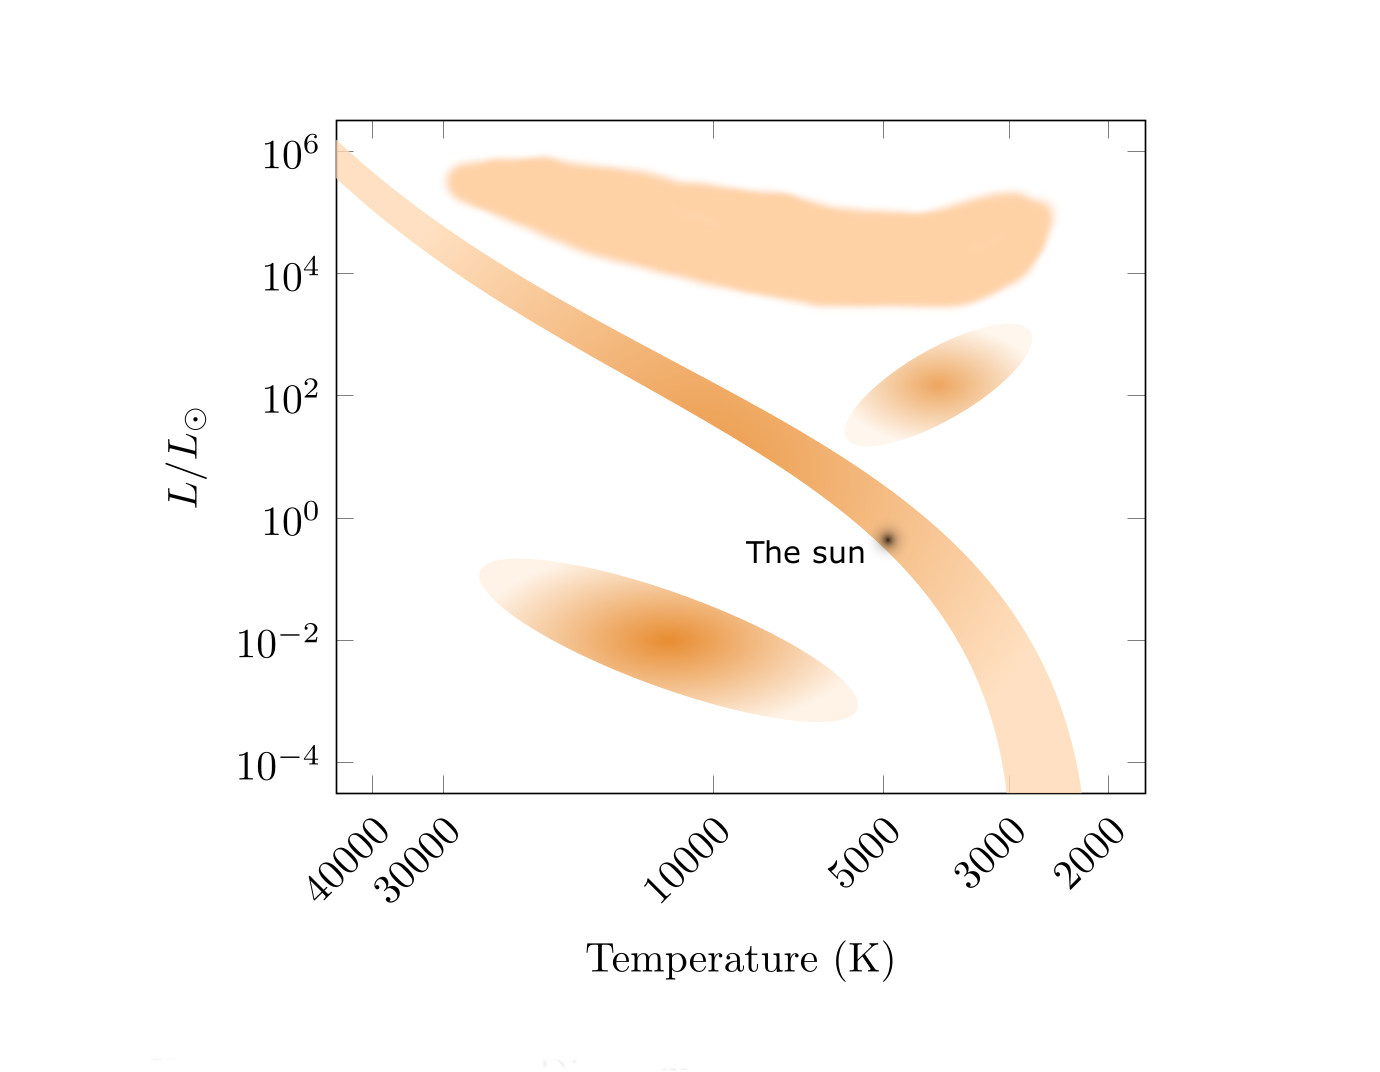
\includegraphics{HR_diagram.jpg}
\end{center}
\vspace{5cm}
\qpart
\begin{center}
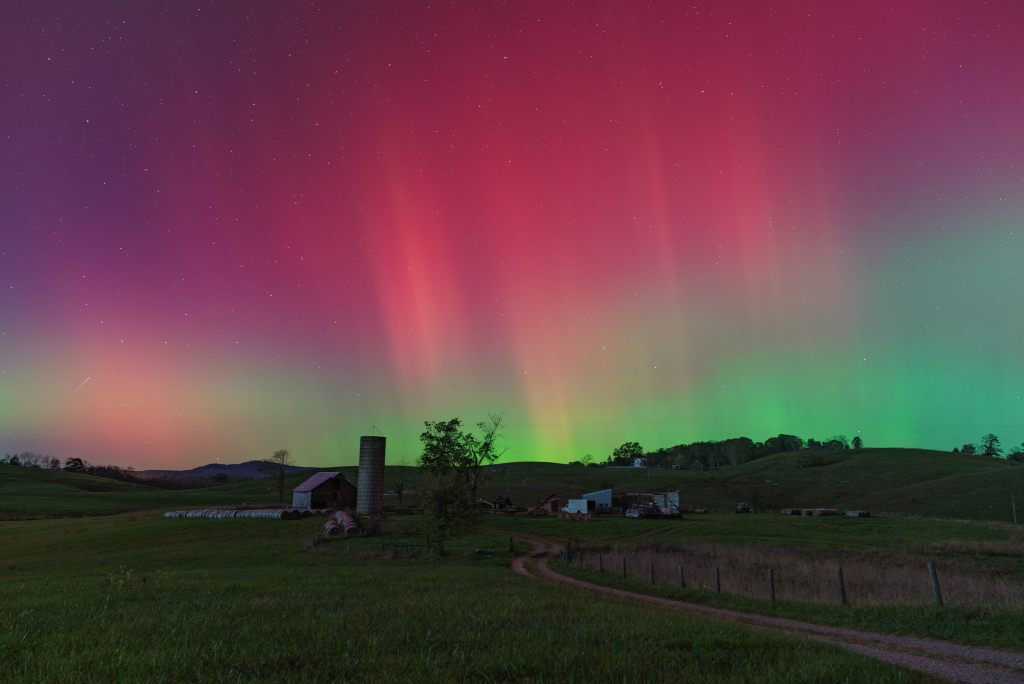
\includegraphics{Pic_of_day.jpeg}
\end{center}
\vspace{5cm}
\qpart
\begin{center}
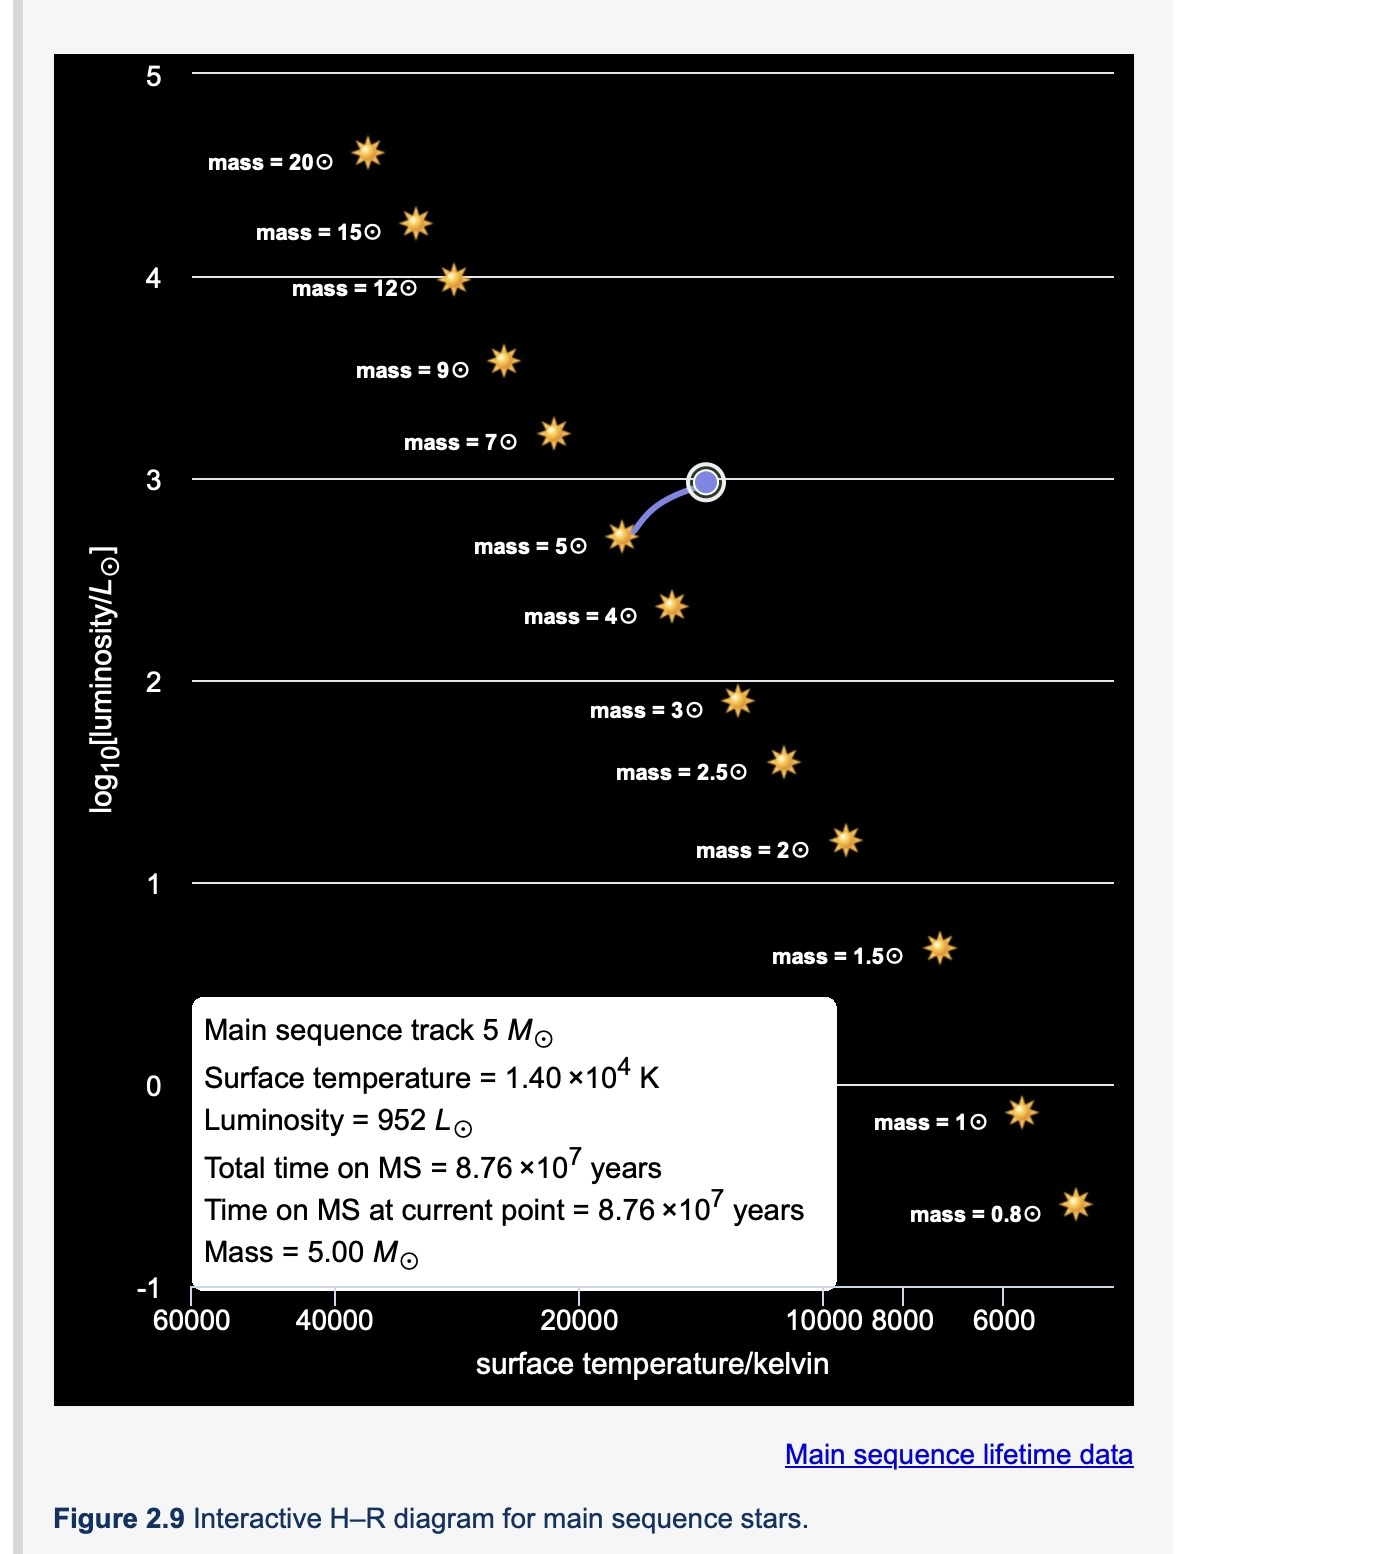
\includegraphics[scale=0.5]{screenshot.jpg}
\end{center}
Investigating the properties of stars on the main sequence, Copyright © 2023, The Open University, Available at: \url{https://learn2.open.ac.uk/mod/oucontent/view.php?id=2288312&section=2.2.1} (13/10/24)
\end{question}

\begin{question}
\begin{center}
\begin{tabular}{lrr}
\arrayrulecolor{blue!20!white}\hline
\rowcolor{blue!20!white}Star & Apparent magnitude($m$) & Distance ($d/pc$)\\
\arrayrulecolor{blue!20!white}\hline
Alpha Cygni & 1.25 & 800\\ 
\arrayrulecolor{blue!20!white}\hline
Beta Cygni & 2.93 & 130\\
\arrayrulecolor{blue!20!white}\hline
Gamma Cygni & 2.23 & 560\\
\arrayrulecolor{blue!20!white}\hline
Delta Cygni & 2.87 & 51\\
\arrayrulecolor{blue!20!white}\hline
Epsilon Cygni & 2.48 & 22\\
\arrayrulecolor{blue!20!white}\hline
\end{tabular}
\end{center}
\end{question}

\begin{question}

\begin{figure}
\centering
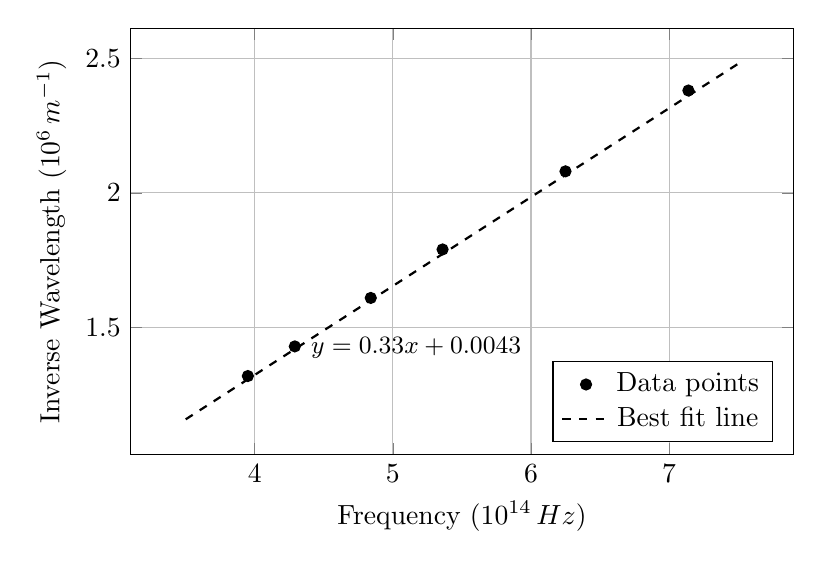
\begin{tikzpicture}
    \begin{axis}[
        xlabel={Frequency ($10^{14} \, \text{Hz}$)},
        ylabel={Inverse Wavelength ($10^6 \, \text{m}^{-1}$)},
        grid=both,
        width=10cm,
        height=7cm,
        legend pos=south east
    ]
    % Data points
    \addplot[
        only marks,
        mark=*,
        mark size=2pt
    ] coordinates {
        (7.14, 2.38)
        (6.25, 2.08)
        (5.36, 1.79)
        (4.84, 1.61)
        (4.29, 1.43)
        (3.95, 1.32)
    };

    % Line of best fit
    \addplot[
        domain=3.5:7.5, % Adjust the domain for the fit line
        samples=100,
        thick,
        dashed
    ]{0.33*x + 0.0043};

    \legend{Data points, Best fit line}
     \node at (axis cs: 6, 1.5) [anchor=north east] {\small$y = 0.33x + 0.0043$};
    
    \end{axis}
\end{tikzpicture}
\caption{Plot of inverse wavelength versus frequency with a best fit line}
\end{figure}

$paulallen@Pauls-Air TMA 00$\\
 $ python3 line_of_best_fit.py$\\
$Slope: 0.3325256100466257$\\
$Intercept: 0.004284972035984325$

\begin{equation}
\begin{split}
c=\lambda f\\
f =\frac{c}{\lambda}\\
\frac{1}{\lambda}=\frac{f}{c}
\end{split}
\end{equation}
Using; \[c \approx \frac{1}{gradient} \approx \SI{3.01e8}{\meter\per\second} \]
\end{question}


\end{document}